% LaTeX path to the root directory of the current project, from the directory in which this file resides
\providecommand{\econtexRoot}{}\renewcommand{\econtexRoot}{.}
\providecommand{\econtexPaths}{LaTeX}\renewcommand{\econtexPaths}{\econtexRoot/\econtexPaths}

\documentclass[../BufferStockTheory.tex]{subfiles}% LaTeX path to the root directory of the current project, from the directory in which this file resides
\providecommand{\econtexRoot}{}\renewcommand{\econtexRoot}{.}
\providecommand{\econtexPaths}{LaTeX}\renewcommand{\econtexPaths}{\econtexRoot/\econtexPaths}


\input{\LaTeXFiles/onlyinsubfile.sty}\begin{document}
%\onlyinsubfile{\externaldocument{BufferStockTheory}}

  \subsection{Commutative Diagrams for the Perfect Foresight Model}
The diagrams below illustrate the order of the several conditions in the text:

\tikzset{node distance=6cm, auto, >=latex}
\begin{figure}[tbp]
	\centerline{
		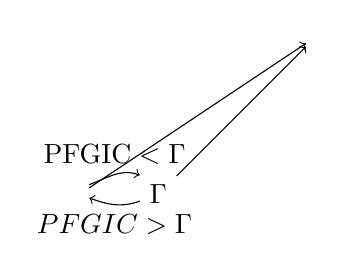
\begin{tikzpicture}
		\node (thorn) {$\textbf{\Thorn}$};
		\node (gamma) [right of = thorn] {$\Gamma$};
		\node (rfree) [below of = thorn, xshift = 3cm, yshift = 
		3cm]{$\mathsf{\Rfree}$};
		
		\draw[->] (thorn.north east) to [out = 20,  in=160] node[above]{$\mathrm{PFGIC} \Thorn < \Gamma$} (gamma.north west);
		\draw[->] (gamma) to [out = 200, in=-20] node[below]{$\cncl{PFGIC} \Thorn  > \Gamma$} (thorn);
		\draw[->] (thorn) to node [swap] {$\mathrm{\RIC}$} (rfree);
		\draw[->] (gamma) to node {$\mathrm{\FHWC}$} (rfree);
		\end{tikzpicture}
	}
\caption{\textcolor{red}{Name of diagram 1}}
\end{figure}
\tikzset{node distance=5cm, auto, >=latex}

and to further incorporate the Perfect Foresight Finite Value of Autarky 
Condition:

\begin{figure}[tbp]
	\centerline{
		\begin{tikzpicture}
		\node (thorn) {$\textbf{\Thorn}$};
		\node (gamma) [right of = thorn] {$\Gamma$};
		\node (rfree) [below of = thorn]{$\mathsf{\Rfree}$};
		\node (pffvacFac) [right of = rfree] 
		{$\mathsf{\Rfree}^{1/\CRRA}\Gamma^{1 - 
				1/\CRRA}$};
		
		\draw[->] (thorn) to node {$\mathrm{\PFGIC}$} (gamma);
		\draw[->] (thorn) to node [swap] {$\mathrm{\RIC}$} (rfree);
		\draw[->] (thorn) to node [swap] {$\mathrm{\PFFVAC}$} (pffvacFac);
		\draw[->] (gamma) to node {$\mathrm{\FHWC}$} (pffvacFac);
		\draw[->] (pffvacFac) to node {$\mathrm{\FHWC}$} (rfree);
		\end{tikzpicture}
	}
	\caption{\textcolor{red}{Name of diagram 2}}
\end{figure}

In both diagrams, an arrow means ``$<$'', which indicates the annotated condition holds, so if a condition is violated, the corresponding arrow is to be reversed. 

These diagrams also keep track of the hierarchy among the conditions. For example, if the right vertical arrow in the second diagram is reversed, then the top right triangle says \PFFVAC + \cncl{\FHWC} implies \PFGIC. If the left vertical arrow is reversed, then \cncl{\RIC} + {\PFGIC} implies \cncl{\FHWC}. 

\begin{figure}[tbp]
	\centerline{
		\begin{tikzpicture}
		\node (thorn) {$\textbf{\Thorn}$};
		\node (gamma) [right of = thorn, xshift = 5cm] {$\Gamma$};
		\node (rfree) [below of = thorn]{$\mathsf{\Rfree}$};
		\node (pffvacFac) [right of = rfree] 
		{$\mathsf{\Rfree}^{1/\CRRA}\Gamma^{1 - 
				1/\CRRA}$};
		\node (pThorn) [left of = thorn] {$\pZero^{1/\rho}\textbf{\Thorn}$};
		\node (compgamma) [above of = gamma, xshift = -5cm, yshift = -2.5cm] 
		{$\PGroAdj$};
		\node (fvacFac) [right of = thorn, yshift = -2cm] 
		{$\mathsf{\Rfree}^{1/\CRRA}\PGrouAdj^{1 
				- 1/\CRRA}$};
		
		\draw[->] (thorn) to node {$\mathrm{\PFGIC}$} (gamma);
		\draw[->] (thorn) to node [swap] {$\mathrm{\RIC}$} (rfree);
		\draw[->] (thorn) to node [swap] {$\mathrm{\PFFVAC}$} (pffvacFac);
		\draw[->] (gamma) to node {$\mathrm{\FHWC}$} (pffvacFac);
		\draw[->] (pffvacFac) to node {$\mathrm{\FHWC}$} (rfree);
		\draw[->] (pThorn) to node {} (thorn);
		\draw[->] (pThorn) to node [swap] {$\mathrm{\WRIC}$} (rfree);
		\draw[->] (gamma) to node {} (compgamma);
		\draw[->] (thorn) to node {$\mathrm{\GIC}$} (compgamma);
		\draw[->] (fvacFac) to node {} (pffvacFac);
		\draw[->] (thorn) to node {$\mathrm{\FVAC}$} (fvacFac);
		\end{tikzpicture}	
	}
	\caption{\textcolor{red}{Name of diagram 3}}
\end{figure}

\onlyinsubfile{\bibliography{\econtexRoot/BufferStockTheory,economics}}

\end{document}
